\section{Introduction}\label{section-introduction}

%$\alpha\beta\gamma\delta\epsilon\varepsilon\zeta\eta\theta\rho\varrho$
%$<\leq\geq>\subset\supset\supseteq\subseteq\pm\mp\times\div\ast\star\circ\cdot$

Hierarchical structures (or trees) frequently occur in information management that required to be stored and retrieved. Common examples of such structure include organization chart, in which positions of an organization are displayed as a tree, and hierarchical file system where files are stored in levels of directories.

Due to the popularity of relational database management systems (RDBMS), it is often required to store hierarchy data in such databases. The first apparent question is how to store hierarchical data in tables of RDMBS, which are great for storing a list of items without much design foresight for storing hierarchical data?

This paper explores ways of storing hierarchical data in relational databases. The goal is to define a few common operations of hierarchical data, the issues of implementing tree structure in relational model, and optimization for these operations.

\section{Definition}\label{section-definition}

\subsection{Tree}\label{section-tree}

Hierarchical data structure is also known as a tree, which is defined as a connected acyclic digraph $G=(V,E)$ of a set of vertices $V$ (also called nodes) and a set of edges $E$ that denotes the relationship between two nodes\footnote{https://en.wikipedia.org/wiki/Tree\_(data\_structure)}. Figure~\ref{fig:tree} depicts a typical tree.

\begin{figure}[h]
\begin{center}
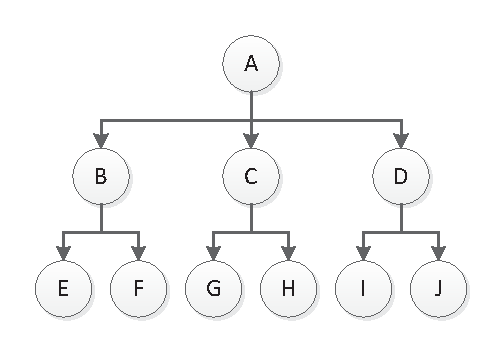
\includegraphics[width=2in]{images/tree.eps}
\caption{Example of a tree.\label{fig:tree}}
\end{center}
\end{figure}

Each node of the tree can hold any number of data item. In the figure above, only identifiers (A--J) of the nodes are shown for simplicity of illustration. The edges of the tree between two nodes are often named children (and sometimes parent) relationship. The relationship is often non-symmetric (as in digraph); for example, $B$ is a child of $A$, but the reverse is not true.

In many literatures of computer data structures, the edges are defined as `children of' a node. For example, node $A$ has children $B$, $C$, and $D$. In the sense of relational database, it does not matter if the edges are defined as `children of' or `parent of'; when one is defined, the other is usually inherited, especially when indexes are used on the relational table in which the tree is stored. The relationship, therefore, will be left for the design of database schema.

\subsection{Relational Database}

Relational data model is proposed by Edgar Codd in 1970\cite{DBLP:journals/cacm/Codd70}. In this model, a database consists of a set of tables (also known as relations), which each consists of a set of tuples. In colloquial usage, tuples are also called records.

Figure~\ref{fig:relational_database} illustrates a relational database with 2 tables, each 3 attributes. The teachers table has 4 records (tuples) and the Courses table has 6.

\begin{figure}[h]
\centering
\subfigure[Teachers Table]{
\label{tab:sample_data_a}
  \begin{tabular}{|c|c|c|}
  \hline
  {\bf ID} & {\bf Name} & {\bf Office} \\ \hline\hline
  1 & James Madison & A\\
  2 & John Adams & B\\
  3 & Ronald Reagan & C\\
  4 & Franklin Pierce & D\\
  \hline
  \end{tabular}}
\subfigure[Courses Table]{
\label{tab:sample_data_a}
  \begin{tabular}{|c|c|c|}
  \hline
  {\bf ID} & {\bf Name} & {\bf Teacher} \\ \hline\hline
  1 & Data Structures & 1\\
  2 & Intro to Algorithms & 1\\
  3 & Software Construction & 2\\
  4 & Computer Networks & 3\\
  5 & Operating Systems & 4\\
  6 & Compilers & 2\\
  \hline
  \end{tabular}}
\caption{A Relational Database\label{fig:relational_database}}
\end{figure}

\subsection{Common Tree Operations}

In this section, we define common operations on trees without considering how the trees are implemented in relational model. Section \ref{sec-nested-set} and \ref{sec-adj-list} will cover implementation details and how these operations are to be performed under these relational designs.

This paper only covers read operations, relyig on the assumption that once an hierarchy is inserted into a database, the structure is rarely changed without removing an entire subtree. Insertion operations are assumed to be done via standard SQL insert statements. Hierarchical update and remove operations are to be covered in future works.

Operations thtat will be used in this paper are enumerated below. All examples use the tree of Figure~\ref{fig:tree}.


%%% Enumeration of operations %%%

\begin{enumerate}

\item $Root(n) \rightarrow r$ : given a node $n$, this operation finds the root $r$ of the tree in which $n$ resides: $Member(n, r) \rightarrow true$.

    \begin{align*}
    & Root(A) \rightarrow A \\
    & Root(E) \rightarrow A
    \end{align*}

    
\item $Parent(n) \rightarrow p$ : Given a node $n$, this operation finds the parent node $p$, or $null$ if $n$ is a root node.

    \begin{align*}
    & Parent(A) \rightarrow  null \\
    & Parent(B) \rightarrow A
    \end{align*}

\item $Children(n) \rightarrow \{c_1, c_2, ..., c_n\}$ : Given a node $n$, this operation finds it's child nodes $\{c_1, c_2, ..., c_n\}$. If $n$ is a leaf node (no children), then the empty set is returned.

    \begin{align*}
    & Children(A) \rightarrow \{B, C, D\} \\
    & Children(E) \rightarrow \{\}
    \end{align*}
    
\item $Siblings(n) \rightarrow \{n_1, n_2, ..., n_n\}$ : This operation finds a list of nodes $\{n_1, n_2, ..., n_n\}$ that have the same depth as node $n$. If this node has no siblings, the empty set is returned.

    \begin{align*}
    & Siblings(A) \rightarrow \{\} \\
    & Siblings(B) \rightarrow \{C, D\}
    \end{align*}

\item $Leaves(n) \rightarrow \{n_1, n_2, ..., n_n\}$ : This operation returns a set of leaf nodes $\{n_1, n_2, ..., n_n\}$ of the subtree rooted at $n$

    \begin{align*}
    & Leaves(A) \rightarrow \{E, F, G, H, I, J\} \\
    & Leaves(B) \rightarrow \{E, F\} \\
    & Leaves(E) \rightarrow \{E\}
    \end{align*}
    
\item $Height(n) \rightarrow \mathbb{N}$ : Given a node $n$, this operation returns the count of node of longest path from $n$ to a leaf node.

    \begin{align*}
    & Height(A) \rightarrow 3 \\
    & Height(E) \rightarrow 1
    \end{align*}
    
\item $Depth(n) \rightarrow \mathbb{N}$ : Given a node $n$, this returns $|Path(n)|$.

    \begin{align*}
    & Depth(A) \rightarrow 1 \\
    & Depth(E) \rightarrow 3 \\
    \end{align*}
    
\item $Path(n) \rightarrow \{n_1, n_2, ..., n_n\}$ : given a node $n$, this operation retrieves the list of nodes $\{n_1, n_2, ..., n_n\}$ that forms the path from root to node $n$, where $n_1$ is the root and $n_n$ is $n$. This operation is the same as retrieving all \emph{ancestors} of $n$.

    \begin{align*}
    & Path(A) \rightarrow \{A\} \\
    & Path(E) \rightarrow \{A, B\}
    \end{align*}
    
\item $Member(n, t) \rightarrow boolean$ : given two nodes $n$ and $t$, this operation tests if node $n$ is a \emph{descendant} of node $t$ -- or, if $n$ is in the subtree rooted at $t$.


    \begin{align*}
    & Member(B, A) \rightarrow true \\
    & Member(A, B) \rightarrow false \\
    & Member(C, B) \rightarrow false
    \end{align*}
    
\item $Tree(n) \rightarrow \{n_1, n_2, ..., n_n\}$ : Gets the hierarchy of the tree

    \begin{align*}
    Depth-first traversal of the tree
    \end{align*}

\end{enumerate} %%% End enumeration of operations %%%


%\section{Tree Representation in Relational Database}

\section{Adjacency List}\label{sec-adj-list}

One of the simplest way of representing hierarchy in relational data model is a method called adjacency list. In this approach, a table (we will call it Nodes table) is used to store the nodes of one or multiple trees, and each record of the table represent a node.

Each record of the Nodes table consists of field of primary key of the identifier of the node, and a field of foreign key that holds the identifier of the parent node, which references the same table. The root node of a tree would have {\em Parent = null}. The schema for the adjacency list table is shown in Figure~\ref{fig:adj_list}.


\begin{figure}[h]
\hrule\vspace{6px}
\begin{verbatim}
CREATE TABLE Nodes (
  ID CHAR PRIMAY KEY NULL,
  Parent CHAR NOT NULL,
  FOREIGN KEY (Parent) REFERENCES Nodes(ID)
)
\end{verbatim}
\hrule
\caption{Schema for adjacency list.\label{fig:adj_list}}
\end{figure}

\begin{remark}[Note:]
The name `adjacency list' may cause a bit of confusion. An adjacency list implies a list of child (adjacent) nodes of a node, but the schema for the table above only has a reference from a node its parent node, which should probably more aptly named `parent-link' approach.

As noted in section~\ref{section-tree}, this distinction is actually not important in relation database. The reason is that with a reference to parent defined, the {\em children} of a node (adjacency list) can be easily found. For example the child nodes of $A$ can be by using the query in Figure~\ref{fig:child_query}:

\begin{figure}[h]
\hrule\vspace{6px}
\begin{verbatim}
SELECT * FROM Nodes WHERE Parent='A'
\end{verbatim}
\hrule
\caption{SQL for querying child nodes.\label{fig:child_query}}
\end{figure}
\end{remark}

\subsection{Operations}

The operation for finding the root node of a tree with a specific node is is trivial. All we need to do is querying for nodes with \emph{Parent = null} and the specific node ID, as shown below:

\begin{figure}[h]
\hrule\vspace{6px}
\begin{verbatim}
SELECT * FROM Nodes WHERE Parent IS NULL
  AND ID='A'
\end{verbatim}
\hrule
\caption{Query for finding the root node for adjacency list method.\label{fig:adj_list_find_root}}
\end{figure}

Operations for finding the parent and children node(s) are also trivial. The query for finding children nodes is already shown in Figure~\ref{fig:child_query}. The following example query finds the parent node of node $B$:

\begin{figure}[h]
\hrule\vspace{6px}
\begin{verbatim}
SELECT Parent FROM Nodes WHERE ID='B'
\end{verbatim}
\hrule
\caption{Query for finding the parent node for adjacency list method.\label{fig:adj_list_find_parent}}
\end{figure}

Although the preceding operations are easy to perform, the drawback of the adjacency list method is that some of the listed operations require multiple queries to be submitted to the database. These operations follows:

\begin{itemize}
\item Member
\item Find Ancestors
\item Find Descendants
\item Get Tree
\end{itemize}

The number of queries of these operations usually depend on the depth of the node in question. Each query submitted to the database incurs communication cost between the processing program and the database; therefore, the cost of computing these operations increases as the depth of the tree increase.

Listing~\ref{member} shows the algorithm for finding if node $B$ is a member of tree $A$. Notice the algorithm issues multiple queries to the database.

\lstset{caption={Algorithm for Member operation},label=member}
\begin{lstlisting}[frame=single]
//Returns true if B is part of Tree A
function Member(char B, char A)
	while(true)
		if(B == A)
			return true
		if(B == null)
			return false
		B = query("SELECT Parent FROM Nodes WHERE ID=B")
\end{lstlisting}

Listing~\ref{AL_PrintTree} shows the recursive algorithm of PrintTree for the adjacency list method.

\begin{minipage}{\linewidth}
\lstset{caption={Algorithm for Member operation},label=AL_PrintTree}
\begin{lstlisting}[frame=single]
PrintTree(char nodeId, int level = 0)
	//Output current node
	for(i = 0 to level)
		Print(' ')
	Print('nodeId')
	
	//Output children
	children = query("SELECT ID FROM Nodes WHERE Parent=" + nodeId)
	foreach(child in children)
		PrintTree(child, level + 1)
\end{lstlisting}	
\end{minipage}

\section{Nested Set}\label{sec-nested-set}

Another way of representing hierarchical data in relational database is the nested set model\cite{journals/trj/Kamfonas92}. This model is an extension of the adjacency list model. The goal of this model is to eliminate the need to issue multiple queries to the database (and the use of recursion) by placing ordering on the nodes. Listing~\ref{ns_schema} shows the relational schema for the nested set model.

\begin{minipage}{\linewidth}
\lstset{caption={Nodes table for nested set model},label=ns_schema}
\begin{lstlisting}[frame=single]
CREATE TABLE Nodes (
    ID CHAR PRIMARY KEY NOT NULL,
    Parent CHAR NULL,
    Left INT NOT NULL,
    Right INT NOT NULL,
    FOREIGN KEY (Parent) REFERENCES Nodes (ID)
)
\end{lstlisting}	
\end{minipage}

In this model, there are, for each node, two additional fields: Left and Right values. These two values provides an ordering of nodes in a tree. Algorithm for assigning left and right value for nodes is shown in Listing~\ref{ns_lr}.

\begin{minipage}{\linewidth}
\lstset{caption={Algorithm for Left-Right value assignment for nested set model},label=ns_lr}
\begin{lstlisting}[frame=single]
int LROrder(Node node, int count = 1)
	n.left = count
	foreach(child in Children(node))
		count = LROrder(child, count + 1)
	n.right = count++
	return count
\end{lstlisting}	
\end{minipage}

The following steps summarizes LROrder algorithm:

\begin{enumerate}
\item Assign $count$ to the $left$ of current node $n$.
\item For each child of node $n$, call LROrder for that child.
\item After the LROrder call is complete for each child, increment and assign $count$ to the right value of current node $n$.
\item Return $count$
\end{enumerate}

Figure~\ref{fig:tree-lr} shows the left-right values for the tree in the Figure~\ref{fig:tree} via the algorithm above.

\begin{figure}[H]
\begin{center}
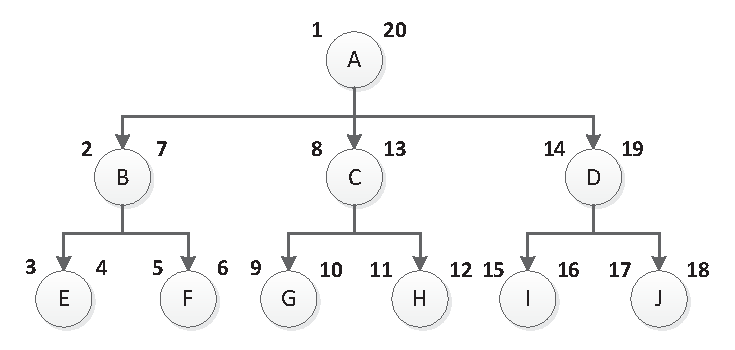
\includegraphics[width=3.3in]{images/tree-lr.eps}
\caption{Example of a tree in nested set model.\label{fig:tree-lr}}
\end{center}
\end{figure}

\subsection{Operations}

\subsubsection{Ancestors}

With nested set model, finding ancestors of a node becomes trivial. Because the left-value of a node is assigned before any child-node is traversed and the right-value after, any \emph{ancestor}, denoted by $a$, of a node $n$ has the following properties:

\begin{enumerate}
\item $a.left < n.left$
\item $n.right < a.right$
\end{enumerate}

\textbf{Note:} ``left'' and ``right'' are SQL keywords, consider changing left to another name.\\

With the above properties, the queries for ancestors no longer require multiple queries (or recursion). Listing~\ref{ns_ancestors} shows the query to get ancestors of node $E$ in Figure~\ref{fig:tree-lr}.

\begin{minipage}{\linewidth}
\lstset{caption={Query for ancestors for node $E$ via nested set model},label=ns_ancestors}
\begin{lstlisting}[frame=single]
SELECT * FROM Nested_Set WHERE Left < 3 AND Right > 4
\end{lstlisting}	
\end{minipage}

\subsubsection{Tree}

Getting the entire hierarchy of a tree is the same as getting all the descendants of the root node (including the root). If the database contains only one tree, then this operation involves retrieving all entries in the nodes table. However, we assume that the database contains multiple disconnected trees.

Listing~\ref{ns-tree} shows this query for the tree in Figure~\ref{fig:tree-lr}, in which the left and right value for the root node $A$ is 1 and 20, respectively.

\begin{minipage}{\linewidth}
\lstset{caption={Query for Tree for tree $A$ via nested set model},label=ns-tree}
\begin{lstlisting}[frame=single]
SELECT * FROM Nested_Set WHERE Left > 1 AND Right < 20 ORDER BY left ASC
\end{lstlisting}	
\end{minipage}

To reconstruct the hierarchical structure from the flat list returned from the query above, we look at the result of the query (of the tree in Figure~\ref{ns-tree}) in the Table~\ref{table:ns_tree} below.

\begin{table}[h]
\centering
\begin{tabular}{|l|l|l|l|}
\hline
{\bf ID} & {\bf Left} & {\bf Right} & {\bf Parent} \\ \hline\hline
A & 1 & 20 & null \\ \hline
B & 2 & 7 & A \\ \hline
E & 3 & 4 & B \\ \hline
F & 5 & 6 & B \\ \hline
C & 8 & 13 & A \\ \hline
G & 9 & 10 & C \\ \hline
H & 11 & 12	& C \\ \hline
D & 14 & 19	& A \\ \hline
I & 15 & 16	& D \\ \hline
J & 17 & 18	& D \\ \hline
\end{tabular}
\caption{Query result of Tree operation\label{table:ns_tree}}
\end{table}

There are two ways to reconstruct the tree, since there are redundant information in the result table to reconstruct the tree. The first way is to only use the `Parent' column. The second way is to use only the `Left' and `Right' columns (not needing the `Parent' column). Listing~\ref{ns_tree_const1} shows the algorithm for the first approach.

\begin{minipage}{\linewidth}
\lstset{caption={Tree reconstruction using Parent},label=ns_tree_const1}
\begin{lstlisting}[frame=single]
Node ReconstructTree(List<Record> records)
	Node root, current = null
	foreach(Record record in records)
		if(current == null)
			current = MakeNode(record)
			root = current
		else
			while(current.ID != record["Parent"])
				current = current.Parent
			Node node = MakeNode(record)
			current.Children.Add(node)
			current = node
	return root
\end{lstlisting}	
\end{minipage}

Listing~\ref{ns_tree_const2} shows the algorithm for the second approach.

\begin{minipage}{\linewidth}
\lstset{caption={Tree reconstruction using Left and Right value},label=ns_tree_const2}
\begin{lstlisting}[frame=single]
//Returns the root node as the tree
Node ReconstructTree(List<Record> records)
	Node root, current = null
	foreach(Record record in records)
		if(current == null) //This should only be run once
			current = MakeNode(record)
			root = current
		else
			while(!(current.Left < record["Left"] and current.Right > record["Right"]))
				current = current.Parent
			Node node = MakeNode(record)
			current.Children.Add(node)
			current = node
	return root
\end{lstlisting}	
\end{minipage}
\subsubsection{Print Tree}

The tree structure can be easily outputted by a program after the hierarchy has been reconstructed with the algorithms in the previous section. However, sometimes a tree has large number of nodes and we may only need to output the tree structure without needing to reconstruct the tree in memory.

This section shows an algorithm to print the ID of the nodes with increasing indention to show the hierarchy of the tree.

\begin{minipage}{\linewidth}
\lstset{caption={Tree reconstruction using Left and Right value},label=ns_print_tree}
\begin{lstlisting}[frame=single]
void PrintTree(List<Record> records)
	//Make new stack to hold right values; 
	//length = 0
	Stack stack;
	foreach(Record record in records)
		while(stack.top < record["right"] and !stack.isEmpty)
			stack.pop()
		//Print identation
		for(int i = 0 to stack.length - 1) 
			Print(" ")
		//Print current record
		Print(Record.ID)
		stack.push(record["right"])
\end{lstlisting}	
\end{minipage}
